%% Except where otherwise noted, content in this documentation is Copyright (c)
%% 2015-2019, RTE (http://www.rte-france.com) and licensed under a
%% CC-BY-4.0 (https://creativecommons.org/licenses/by/4.0/)
%% license. All rights reserved.

\documentclass[a4paper, 12pt]{report}

% Latex setup
%%  Copyright (c) 2015-2019, RTE (http://www.rte-france.com)
%%  See AUTHORS.txt
%%  All rights reserved.
%%  This Source Code Form is subject to the terms of the Mozilla Public
%%  License, v. 2.0. If a copy of the MPL was not distributed with this
%%  file, you can obtain one at http://mozilla.org/MPL/2.0/.
%%  SPDX-License-Identifier: MPL-2.0
%%
%%  This file is part of Dynawo, an hybrid C++/Modelica open source time domain
%%  simulation tool for power systems.


%%%%%%%%%%%%%%%%%%%%%%%%%%%%%%%%%%%%%%%%%%%
% Define text and document settings
%%%%%%%%%%%%%%%%%%%%%%%%%%%%%%%%%%%%%%%%%%%

\usepackage{lmodern} % Latin Modern fam­ily of fonts
\usepackage[english]{babel} % English

% Specify encoding
\usepackage[utf8]{inputenc} % Input
\usepackage[T1]{fontenc} % Output

% Document structure setup
\usepackage{titlesec} % To change chapter format
\setcounter{tocdepth}{3} % Add subsubsection in Content
\setcounter{secnumdepth}{3} % Add numbering for subsubsection
\setlength{\parindent}{0pt} % No paragraph indentation

% Avoid numbering starting at each chapter for figures
\usepackage{chngcntr}
\counterwithout{figure}{chapter}

% Change title format for chapter
\titleformat{\chapter}{\Huge\bf}{\thechapter}{20pt}{\Huge\bf}

% To add links on page number in Content and hide red rectangle on links
\usepackage[hidelinks, linktoc=all]{hyperref}
\usepackage[nottoc]{tocbibind} % To add biblio in table of content
\usepackage{textcomp} % For single quote
\usepackage{url} % Allow linebreaks in \url command
\usepackage{listings} % To add code samples

% Define typography
\usepackage{xspace}
\usepackage{dirtree}
\newcommand{\Dynawo}[0]{Dyna$\omega$o\xspace}

% Default listings parameters
\lstset
{
  aboveskip={1\baselineskip}, % A bit of space above
  backgroundcolor=\color{shadecolor}, % Choose the background color
  basicstyle={\ttfamily\footnotesize}, % Use font and smaller size \small \footnotesize
  breakatwhitespace=true, % Sets if automatic breaks should only happen at whitespace
  breaklines=true, % Sets automatic line breaking
  columns=fixed, % Nice spacing -> fixed / flexible
  mathescape=false, % Escape to latex false
  numbers=left, % Where to put the line-numbers
  numberstyle=\tiny\color{gray}, % The style that is used for the line-numbers
  showstringspaces=false, % Do not emphasize spaces in strings
  tabsize=4, % Number of spaces of a TAB
  texcl=false, % Activates or deactivates LaTeX comment lines
  upquote=true % Upright quotes
}

%%%%%%%%%%%%%%%%%%%%%%%%%%%%%%%%%%%%%%%%%%%
% Define plots settings
%%%%%%%%%%%%%%%%%%%%%%%%%%%%%%%%%%%%%%%%%%%

% Macro pack­age for cre­at­ing graph­ics
\usepackage{tikz}
\usepackage{subfigure}
\usepackage{float}

% Draws func­tion plots (based on pgf/tikz)
\usepackage{pgfplots}
\pgfplotsset{enlarge x limits=false, xlabel={\begin{small}$time$ (s)\end{small}}, height=0.6\textwidth, width=1\textwidth}
\pgfplotstableset{col sep=semicolon}

% Define colors
\usepackage{color}
\definecolor{blue}{rgb}{.3,.5,1}
\definecolor{deepblue}{rgb}{0,0,1}
\definecolor{darkblue}{rgb}{0,0,.4}
\definecolor{red}{rgb}{1,0,0}
\definecolor{darkred}{rgb}{.56,0,0}
\definecolor{pink}{rgb}{.933,0,.933}
\definecolor{purple}{rgb}{0.58,0,0.82}
\definecolor{green}{rgb}{0.133,0.545,0.133}
\definecolor{darkgreen}{rgb}{0,.4,0}
\definecolor{gray}{rgb}{.3,.3,.3}
\definecolor{darkgray}{rgb}{.2,.2,.2}
\definecolor{shadecolor}{gray}{0.925}

%%%%%%%%%%%%%%%%%%%%%%%%%%%%%%%%%%%%%%%%%%%
% Define blocks for simple network drawings
%%%%%%%%%%%%%%%%%%%%%%%%%%%%%%%%%%%%%%%%%%%

% Define blocks for newtorks drawings
\usepackage{amsmath} % Add math­e­mat­i­cal fea­tures
\usepackage{schemabloc} % Add block diagram library (french one)

%% Define infinite bus
\tikzset{infinite bus/.pic={
  code={
  \draw (0,0) circle (2) node[inner sep=0, outer sep=0] {{$\infty$}};
  \draw (2,0) --++ (2,0);
  }
  }
}

%% Define transformer
\tikzset{transfo/.pic={
  code={
  \draw (0,0) circle (2);
  \draw (2,0) circle (2);
  \draw (4,0) --++ (4,0);
  \draw (-2,0) --++ (-4,0);
  }
  }
}

%% Define generator
\tikzset{generator/.pic={
  code={
    \draw (0,0) circle (2);
    \draw (0,0) arc (0:180:0.5);
    \draw (0,0) arc (180:360:0.5);
    \draw (-2,0) --++ (-2,0);
  }
  }
}

%% Define generator controls
\tikzset{VR/.pic={
  code={
  \draw (0,0) circle (2) node[inner sep=0, outer sep=0] {{VR}};
  }
  }
}

%% Define SVarC
\tikzset{SVarC/.pic={
  code={
  \draw (0,0) circle (4) node[inner sep=0, outer sep=0] {{SVarC}};
  }
  }
}


\begin{document}

\title{\Dynawo Installation Documentation}
\date\today

\maketitle
\tableofcontents

\chapter{Install procedure}

\section{Building requirements on Unix/Linux}

For the moment \Dynawo has only be tested on Linux platforms (Centos and Debian based) and provided that you can install system packages there should be no problem on other Linux distribution. For MacOS and Windows users a \href{https://www.docker.com/}{\underline{Docker}} solution will be provided in a near future. We also plan to provide compilation compatibility for Windows.

In the following we give a list of requirements needed to build \Dynawo and its dependencies.

\paragraph{Global}

\begin{itemize}
\item Compilers: C and C++ (\href{https://www.gnu.org/software/gcc}{gcc} or \href{https://clang.llvm.org}{clang}), c++98 or c++11 compatible for C++ standard
\end{itemize}

\paragraph{OpenModelica Compiler}

\begin{itemize}
\item
  Compiler: Fortran (\href{https://gcc.gnu.org/fortran/}{gfortran})
\item
  Build systems:
  \href{https://www.gnu.org/software/autoconf/}{autoconf},
  \href{https://www.gnu.org/software/autoconf/}{automake},
  \href{https://www.gnu.org/software/libtool/}{libtool},
  \href{http://pkgconf.org/}{pkgconf}, make,
  \href{https://cmake.org/}{CMake}
\item
  Binary utilities: \href{https://tukaani.org/xz/}{xz}, patch,
  \href{https://www.gnu.org/software/sed/}{GNU sed}, msgfmt from
  \href{https://www.gnu.org/software/gettext/}{gettext},
  \href{https://rsync.samba.org/}{rsync}
\item
  Java (\href{https://openjdk.java.net/}{openjdk} for example)
\item
  Libraries: \href{https://libexpat.github.io/}{expat},
  \href{http://www.netlib.org/blas/index.html}{BLAS},
  \href{http://www.netlib.org/lapack/index.html}{LAPACK}
\item
  \href{http://lpsolve.sourceforge.net/}{lpsolve55} or
  \href{https://www.gnu.org/software/bison/}{bison} and
  \href{https://www.gnu.org/software/flex/}{flex} (to let OpenModelica
  compiles lpsolve itself)
\end{itemize}

\paragraph{\Dynawo user}

\begin{itemize}
\item
  \href{https://cmake.org/}{CMake}: minimum version 3.9.6 (last version
  to compile with c++98 compiler)
\item
  Libraries:

  \begin{itemize}
  \item
    \href{https://www.libarchive.org/}{libarchive}: minimum version
    2.8.0, latest 3.3.3 version has been tested and works fine
  \item
    \href{https://www.boost.org/}{Boost}: minimum version 1.59, up to
    1.69 multiple versions have been tested and work fine
  \end{itemize}

\item
  Python
\item
  Python packages: \href{https://lxml.de/}{lxml}
\item
  Binary utilities: \href{https://curl.haxx.se/}{curl} or
  \href{https://www.gnu.org/software/wget/}{wget},
  \href{http://xmlsoft.org/xmllint.html}{xmllint}
\end{itemize}

\paragraph{\Dynawo developer}

\begin{itemize}
\item
  \href{http://www.doxygen.nl/}{Doxygen}: minimum version 1.8,
  \href{https://graphviz.readthedocs.io/en/stable/}{Graphviz} and LaTeX
  to build full documentation
\item
  Python packages:
  \href{https://psutil.readthedocs.io/en/latest/}{psutil}
\item
  \href{https://github.com/google/googletest}{GoogleTest}: minimum
  version 1.5.0, latest 1.8.1 version has been tested and works fine on
  recent OS
\item
  \href{http://ltp.sourceforge.net/coverage/lcov.php}{LCOV}: 1.7 to 1.13
  versions work fine
\end{itemize}

\section[Building Dynawo]{Building \Dynawo}
\label{Dynawo_Installation_Documentation_Building_Dynawo}

You can install the following packages to have no dependency problem in the following steps. This example works for Ubuntu: \\

Command for Ubuntu:

\begin{lstlisting}[language=bash]
$> apt-get install -y git gcc g++ gfortran autoconf pkgconf automake make libtool cmake hwloc openjdk-8-jdk libblas-dev liblpsolve55-dev libarchive-dev doxygen doxygen-latex liblapack-dev libexpat1-dev libsqlite3-dev libxerces-c-dev zlib1g-dev gettext patch clang python-pip libncurses5-dev libreadline-dev libdigest-perl-md5-perl unzip gcovr lcov libboost-all-dev qt4-qmake qt4-dev-tools lsb-release libxml2-utils python-lxml python-psutil wget libcurl4-openssl-dev rsync
\end{lstlisting}

Command for Fedora:

\begin{lstlisting}[language=bash]
$> dnf install -y git gcc gcc-c++ gcc-gfortran autoconf automake make libtool cmake hwloc java-1.8.0-openjdk-devel blas-devel lapack-devel lpsolve-devel expat-devel glibc-devel sqlite-devel xerces-c-devel libarchive-devel zlib-devel doxygen doxygen-latex qt-devel gettext patch wget python-devel clang llvm-devel ncurses-devel readline-devel unzip perl-Digest-MD5 vim gcovr python-pip python-psutil boost-devel lcov gtest-devel gmock-devel xz rsync python-lxml graphviz libcurl-devel
\end{lstlisting}

To build \Dynawo you need to clone its repository and launch the following commands in the source code directory:

\begin{lstlisting}[language=bash]
$> git clone https://github.com/dynawo/dynawo.git dynawo
$> cd dynawo
$> echo '#!/bin/bash
export DYNAWO_HOME=$(cd "$(dirname "${BASH_SOURCE[0]}")" && pwd)

export SRC_OPENMODELICA=$DYNAWO_HOME/OpenModelica/Source
export INSTALL_OPENMODELICA=$DYNAWO_HOME/OpenModelica/Install

export DYNAWO_LOCALE=en_GB
export RESULTS_SHOW=true
export BROWSER=xdg-open

export NB_PROCESSORS_USED=$(($(nproc --all) / 2))

export BUILD_TYPE=Release
export CXX11_ENABLED=YES

$DYNAWO_HOME/util/envDynawo.sh $@' > myEnvDynawo.sh
$> chmod +x myEnvDynawo.sh
$> ./myEnvDynawo.sh build-user
\end{lstlisting}

Below is a description of some environment variables that might be changed in the file \textit{myEnvDynawo.sh}:

\begin{center}
\begin{tabular}{|l|l|}
  \hline
   BROWSER & Default browser command \\
  \hline
   NB\_PROCESSORS\_USED & Maximum number of cores to use \\
  \hline
   BUILD\_TYPE & Build type : Release or Debug \\
  \hline
\end{tabular}
\end{center}

We advise the user to install an autocompletion script to help you with the available commands in \Dynawo. I will also add an alias to your bashrc or zshrc to be able to execute \Dynawo from anywhere. You can launch one of the following commands:
\begin{lstlisting}[language=bash,deletekeywords={help,source}]
$> ./myEnvDynawo.sh deploy-autocompletion --deploy --shell-type bash
$> ./myEnvDynawo.sh deploy-autocompletion --deploy --shell-type zsh
\end{lstlisting}

\textbf{Warning}: If you're working behind a proxy make sure you have exported the following proxy environment variables:

\begin{lstlisting}[language=bash]
$> export http_proxy=
$> export https_proxy=
$> export no_proxy=localhost,127.0.0.0/8,::1
$> export HTTP_PROXY=$http_proxy;export HTTPS_PROXY=$https_proxy;export NO_PROXY=$no_proxy;
\end{lstlisting}

\section[Launching Dynawo]{Launching \Dynawo}

Once you have installed and compiled \Dynawo as explained in part \ref{Dynawo_Installation_Documentation_Building _Dynawo}, you can launch a simulation by calling:

\begin{lstlisting}[language=bash, breaklines=true, breakatwhitespace=false]
$> ./myEnvDynawo.sh jobs nrt/data/IEEE14/IEEE14_BasicTestCases/IEEE14_DisconnectLine/IEEE14.jobs
\end{lstlisting}

This command launches a simple simulation on the IEEE 14-bus network that should succeed if your installation went well and your compilation finished successfully.

The correctness of the simulation can be checked by looking into the outputs directory and compare its content with the ones from the reference outputs directory (especially the curves file).

\begin{lstlisting}[language=bash, breaklines=true, breakatwhitespace=false]
$> cd nrt/data/IEEE14/IEEE14_BasicTestCases/IEEE14_DisconnectLine
$> ls outputs
$> diff outputs/curves/curves.csv reference/outputs/curves/curves.csv
\end{lstlisting}

All the simulation outputs are stored into the outputs directory, as specified in the jobs file. \\

It is also possible to display directly simulation results - plots - into a simple GUI (created for demonstration purpose) by using for example the following command:

\begin{lstlisting}[language=bash, breaklines=true, breakatwhitespace=false]
$> ./myEnvDynawo.sh jobs-with-curves nrt/data/IEEE14/IEEE14_BasicTestCases/IEEE14_DisconnectLine/IEEE14.jobs
\end{lstlisting}

For example, for this line disconnection simulation, on Figure~\ref{IEEE14DisconnectLine} we can see the plot for the voltage module in p.u. on bus 10.

\begin{figure}[h!]
\centering
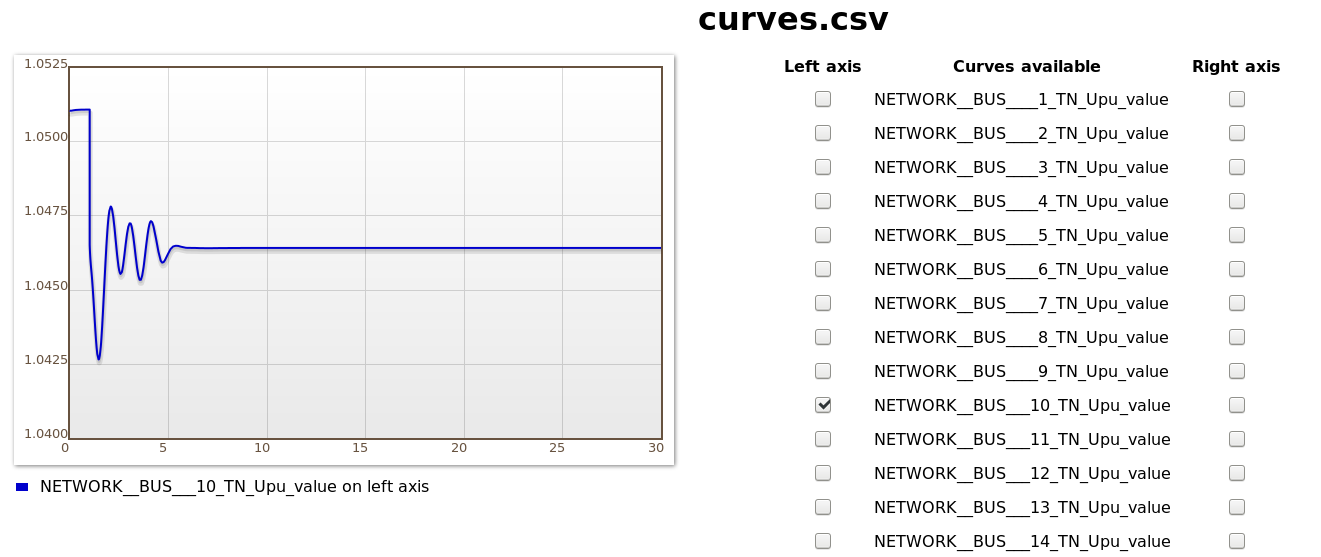
\includegraphics[width=\textwidth]{../resources/VoltageModule.png}
\caption{\Dynawo results on IEEE14\_DisconnectLine case}
\label{IEEE14DisconnectLine}
\end{figure}

\section{Third parties}

To run a simulation, \Dynawo uses several external libraries that are downloaded and compiled during the building process:
\begin{itemize}
\item \href{https://www.openmodelica.org/} {\underline{OpenModelica}} \cite{openmodelica}, a Modelica \cite{modelica} environment developed and maintained by the Open Source Modelica Consortium distributed under a GPL V3.0 or OSMC Public License V1.2. \Dynawo is currently using the version 1.9.4 of the OpenModelica compiler to compile Modelica models either at run-time or beforehand during the compilation process. OpenModelica compiler source code is modified to match specific needs from \Dynawo ; these modifications are available in \path|dynawo/3rdParty/omcUpdate_1_9_4|.

\item \href{https://computation.llnl.gov/projects/sundials}{\underline{SUNDIALS}} \cite{hindmarsh2005sundials}, a suite of solvers developed and maintained by the Lawrence Livermore National Lab distributed under a BSD-3-Clause license. \newline \Dynawo is currently using the version 4.1.0 from SUNDIALS. Small modifications on the library are applied to fit \Dynawo's needs and are available in \path|dynawo/3rdParty/sundials|. In particular, KINSOL and IDA from the SUNDIALS library are called to solve the Algebraic Equations and Differential Algebraic Equations systems arising during the simulation.

\item \href{http://faculty.cse.tamu.edu/davis/suitesparse.html} {\underline{SuiteSparse}}, a suite of sparse matrix algorithms and in particular KLU \cite{DavisKLU}, a LU decomposition library that is  developed and maintained by T. A. Davis et al. at the University of Florida. \Dynawo currently uses the V 4.5.4 version of the suite sparse library that is distributed under a LGPL-2.1+ license. KLU is used inside KINSOL and IDA to make the LU decomposition required during Newton-Raphson resolutions.

\item \href{http://www.met.reading.ac.uk/clouds/adept/}{\underline{Adept}} \cite{hogan_robin_j_2017_1004730} \cite{Hogan:2014:FRA:2639949.2560359}, an automatic differentiation library that is developed and maintained at the University of Reading by R.J. Hogan. The 2.0.5 version is currently employed into \Dynawo to evaluate the Jacobian matrices for Modelica models during the simulation and distributed under both Apache-2.0, GPL-2.0 and MIT licenses.

\item \href{http://xerces.apache.org/xerces-c/}{\underline{Xerces-C++}} a validating XML parser written in a portable subset of C++ and distributed under the Apache Software License, Version 2.0. The current version used is 3.2.2.

\item \href{http://nicslu.weebly.com/} {\underline{NICSLU}} \cite{chenNicsLu} which is another LU decomposition library. It is developed and maintained by Tsinghua University and is optional at the moment into \Dynawo .If downloaded by the user, it could be used for LU decomposition in a similar way than KLU. This library is distributed under GNU LGPL license for open-source projects.
\end{itemize}

In addition to these libraries needed for the simulation process, \Dynawo downloads the code for two other libraries:
\begin{itemize}
\item \href{https://jquery.com/}{\underline{jQuery}} is used to provide a minimalistic GUI with \Dynawo that enables to visualize the results into a browser. jQuery is distributed under both a MIT and GPL license.
\item \href{https://github.com/google/styleguide/tree/gh-pages/cpplint}{\underline{cpplint}}, a tool used during \Dynawo compilation process to ensure that the C++ files follow the Google\textquotesingle s C++ style.
\end{itemize}

Finally, \Dynawo also uses a large number of other system libraries for its compilation process, the unit testing process or to build its source documentation. These libraries must be installed by the developer before compiling \Dynawo and the complete list is given in \ref{Dynawo_Installation_Documentation_Building_Dynawo}.

\bibliography{../resources/dynawoDocumentation}
\bibliographystyle{abbrv}

\end{document}
